% ref: https://tikz.net/blackbody_color/
% author: Izaak Neutelings (March 2019)
\documentclass[border=3pt,tikz]{standalone}
\tikzset{>=latex} % for LaTeX arrow head
\usepackage{xcolor}
\usepackage{physics}
\usepackage{siunitx}

\pgfdeclareverticalshading{rainbow}{100bp}{
  color(0bp)=(red); color(25bp)=(red); color(35bp)=(yellow);
  color(45bp)=(green); color(55bp)=(cyan); color(65bp)=(blue);
  color(75bp)=(violet); color(100bp)=(violet)
}

\pgfdeclareverticalshading{blackbody}{100}{
  rgb(0)=(0,0,0);
  rgb(25)=(0,0,0);
  rgb(25+50/11*1)=(1,0.0337,0);
  rgb(25+50/11*2)=(1,0.2647,0.0033);
  rgb(25+50/11*3)=(1,0.4870,0.1411);
  rgb(25+50/11*4)=(1,0.6636,0.3583);
  rgb(25+50/11*5)=(1,0.7992,0.6045);
  rgb(25+50/11*6)=(1,0.9019,0.8473);
  rgb(25+50/11*6.5)=(1,1,1);
  rgb(25+50/11*7)=(0.9337,0.9150,1);
  rgb(25+50/11*8)=(0.7874,0.8187,1);
  rgb(25+50/11*9)=(0.6925,0.7522,1);
  rgb(25+50/11*10)=(0.6268,0.7039,1);
  rgb(75)=(0.3277,0.5022,1);
  rgb(100)=(0.3277,0.5022,1)
}


\begin{document}


% RAINBOW

\begin{tikzpicture}
  \shade[shading=rainbow,shading angle=270] (0,0) rectangle (10,1);
\end{tikzpicture}


% BLACK BODY
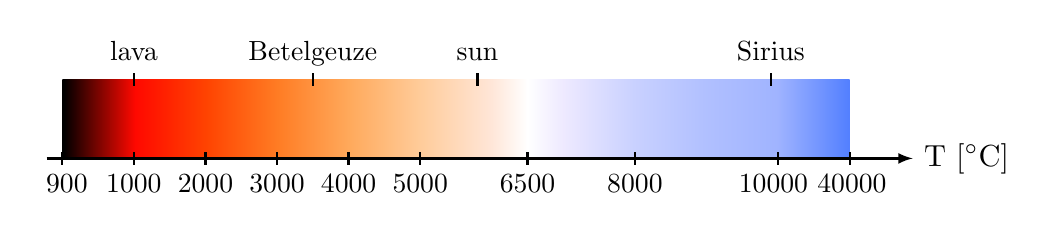
\begin{tikzpicture}
  
  \def\tick#1#2{\draw[thick] (#1+.08) --++ (0,-.16) node[below=-2pt,scale=1] {\strut #2};}
  \def\ticka#1#2{\draw[thick] (#1+.08) --++ (0,-.16) node[above=2pt,scale=1] {\strut #2};}
  
  %   i  TEMPERATURE  RGB COLOR
  %   0        900    0.0000 0.0000 0.0000
  %  10       1000    1.0000 0.0337 0.0000
  %  20       2000    1.0000 0.2647 0.0033
  %  30       3000    1.0000 0.4870 0.1411 
  %  40       4000    1.0000 0.6636 0.3583
  %  50       5000    1.0000 0.7992 0.6045
  %  60       6000    1.0000 0.9019 0.8473
  %           6500    0.9997 0.9998 1.0000 white
  %  70       7000    0.9337 0.9150 1.0000
  %  80       8000    0.7874 0.8187 1.0000
  %  90       9000    0.6925 0.7522 1.0000
  %          10000    0.6268 0.7039 1.0000
  %          15000    0.4749 0.5824 1.0000
  %          30000    0.3751 0.4926 1.0000
  % 100      40000    0.3277 0.5022 1.0000
  % http://www.vendian.org/mncharity/dir3/blackbody/UnstableURLs/bbr_color.html
  
  \shade[shading=blackbody,shading angle=-90] (0,0) rectangle (10,1);
  \draw[->,thick] (-0.2,0) -- (10.8,0) node[right,scale=1.1] {T [\si{\degree C}]};
  \tick{0,0}{ 900}
  \tick{10/11*1,0}{1000}
  \tick{10/11*2,0}{2000}
  \tick{10/11*3,0}{3000}
  \tick{10/11*4,0}{4000}
  \tick{10/11*5,0}{5000}
  \tick{10/11*6.5,0}{6500}
  \tick{10/11*8,0}{8000}
  \tick{10/11*10,0}{10000\,\,}
  \tick{10,0}{\,40000}
  
  % EXAMPLES
  \ticka{10/11*1.0,1}{\strut lava}
  \ticka{10/11*3.5,1}{\strut Betelgeuze}
  \ticka{10/11*5.8,1}{\strut sun}
  \ticka{10/11*9.9,1}{\strut Sirius}
  
\end{tikzpicture}


\end{document}